\documentclass[11pt]{article}
\usepackage{geometry}                % See geometry.pdf to learn the layout options. There are lots.
\geometry{letterpaper}                   % ... or a4paper or a5paper or ... 
%\geometry{landscape}                % Activate for for rotated page geometry
%\usepackage[parfill]{parskip}    % Activate to begin paragraphs with an empty line rather than an indent
\usepackage{graphicx}
\usepackage{amsmath}
\usepackage{amssymb}
\usepackage{url}
\usepackage{epstopdf}
\DeclareGraphicsRule{.tif}{png}{.png}{`convert #1 `dirname #1`/`basename #1 .tif`.png}

%\usepackage{fancyvrb}
%\usepackage{relsize}
%
%\RecustomVerbatimEnvironment
%  {Verbatim}{Verbatim}
%  {fontsize=\relsize{-1},formatcom=\vskip .2cm,samepage}

\title{The Pizza Problem \\ and its illustration of risks with psychological modeling}
\author{Harold Thimbleby}
%\email{harold@thimbleby.net}
\begin{document}
\maketitle

\begin{abstract}
\noindent
A reflection on the unnoticed complexity and unreliability of psychological models (and, by implication, the unreliability of scientific models in general) as motivated by the apparently simple problem, specification, and code openly proposed and illustrated in G Olivia \& A E Martin ``How computational modeling can force theory building in Psychological Science,'' \emph{Perspectives on Psychological Science} %, \textbf{16}(4):789--802, 2021. 
\cite{pizzap}.

\begin{quote}\flushright
--- {\sf Through writing code, we debug our scientific thinking.} \\ G Olivia \& A E Martin, \cite{pizzap}
\end{quote}
\end{abstract}

\section{Introduction}
The Pizza Problem is raised in \cite{pizzap} in the context of arguing that demands of computational modeling guide us toward better science by forcing us to conceptually analyze, specify, and formalize intuitions that may otherwise remain unexamined. A specification and implementation of the Pizza Problem were provided to illustrate the paper. 

Many computer models are complex, even running into tens of thousands or more lines of code \cite{harold-cj}, so discussions of modeling are often eclipsed by the complexity of the domain, the theory, the model, and their assumptions. Often domain theories are extremely complex, for instance expressed as systems of differential equations applied to large data, so refining them into executable models can only be done by making simplifications --- the pragmatic informality introduced in the coding process belies the superficial precision of the theory, and belies the apparent rigor of any published claims based on model results. In contrast, an important aspect of the Pizza Problem discussed here is that it is very simple: the problem itself can be stated in a single sentence, and the mathematics to model it is elementary.

The paper ``Improving science that uses code'' \cite{harold-cj}, within a larger discussion of science that depends on code, points out by way of an example that the Pizza Problem model presented in \cite{pizzap} is incorrect. In the present paper, we carefully examine the model specification and code, and hence discuss the fragility of modeling more generally. 

An important point is that very little of the present discussion could have been developed if the original paper \cite{pizzap} had not openly presented all of the problem, specification, and complete code. Analogously, other work exploring or correcting errors in any science based on computational models is unlikely to be adequate without similar completeness and openness to sharing both specification and code. 

In general, running a computer model promises to improve scrutiny and uncover weaknesses in the model, because the computer runs exactly what it is told, without being biased or motivated for the model to confirm a pet theory. (Sadly scrutiny is often limited to the research team, because the model is not openly shared for independent scrutiny.) The computer itself provides a new sort of scientific scrutiny: a computer runs \emph{exactly\/} what it is told, and human error, including misunderstanding how to correctly implement a model in code, as well as emotively motivated tweaks to the code (often casually introduced during debugging when test results diverge from what was hoped for), combine to ensure that results from running code may be misleading, even deceptive. Often the scientists' models are run on systems developed elsewhere, such as proprietary programming languages or statistics packages, and they are therefore relying on those systems being correct (and correctly documented) --- which they often are not \cite{heedless}. Furthermore, a computer is technically precise in how it runs code, and therefore implemented models may have detailed properties and behavior that require software engineering expertise to ensure is correct, without which na\" \i ve scientists may take, and perhaps write up, an artifact of running a program as an intended consequence of running a poorly-defined or poorly-implemented model.

\section{The Pizza Problem}
The discussion is motivated by a simple problem:

\def\orderA{{\sf\bfseries a}}
\def\orderB{{\sf\bfseries b}}

\begin{quote}\sf
Your favorite pizzeria has a special: two 12 inch pizzas for the price of one 18 inch pizza. Your definition of a good deal is one in which you purchase the most food. Is this a good deal?  \cite{pizzap}
\end{quote}

As the two options are the same price, you can purchase either at the same price, and hence obtain a good deal regardless, assuming at least one of the choices is a good deal. So, since you have a free choice, necessarily, this is a good deal.

A more precise definition of a good deal is perhaps, given that the offer is two choices at the same price, will you choose the larger amount of pizza and not be exploited by being tricked into buying less pizza for the same price? If this is the definition of a good deal, you are still likely to agree it is a good deal, since you \emph{feel\/} free to choose the more generous offer. However you may not realize that you could be deceived: there may be more to this deal that at first it appears. The problem is more subtle than the basic discussion taken from the paper makes it seem. 

Perhaps the offer should be more blatant in the deal the pizzeria is offering --- and hoping to profit from at the customer's expense:

\begin{quote}\begin{center}\sf\framebox[2.75in]{\vbox{~\\Special offer! \\~
\\ Get \textbf{TWO} generous 12 inch pizzas\\ for the price of \textbf{ONE} 18 inch pizza!\\~\\} }
\end{center}\end{quote}

Indeed, even how the question is posed, say whether it arises in a natural encounter in an actual pizzeria, or, at another extreme, in a laboratory with white-coated investigators, would likely induce different or different distributions of answers. The paper \cite{pizzap} reports that expressing the problem on Twitter gained diverse replies, with participants expressing surprise and disbelief at the right answer; even, some tweeted that two pizzas are more than one pizza. Indeed, the question might also be presented in a peer reviewed paper (such as \cite{pizzap} itself) and thereby elicit further types of response. The specific wording and presentation of the problem is a source of different assumptions about the required answer. 

Refer to figure \ref{supplement-fig:pizzas} to consider again which equally-priced choice, order \orderA\ or order \orderB, is the one ``in which you purchase  more food'' (for the same price). 

\begin{figure}[t] 
   \centering
   \begin{tabular}{c@{\hskip 1cm}|@{\hskip 0.7cm}c}
   Order \orderA & Order \orderB\\
   Two 12 inch pizzas & One 18 inch pizza \\  \hline \\
   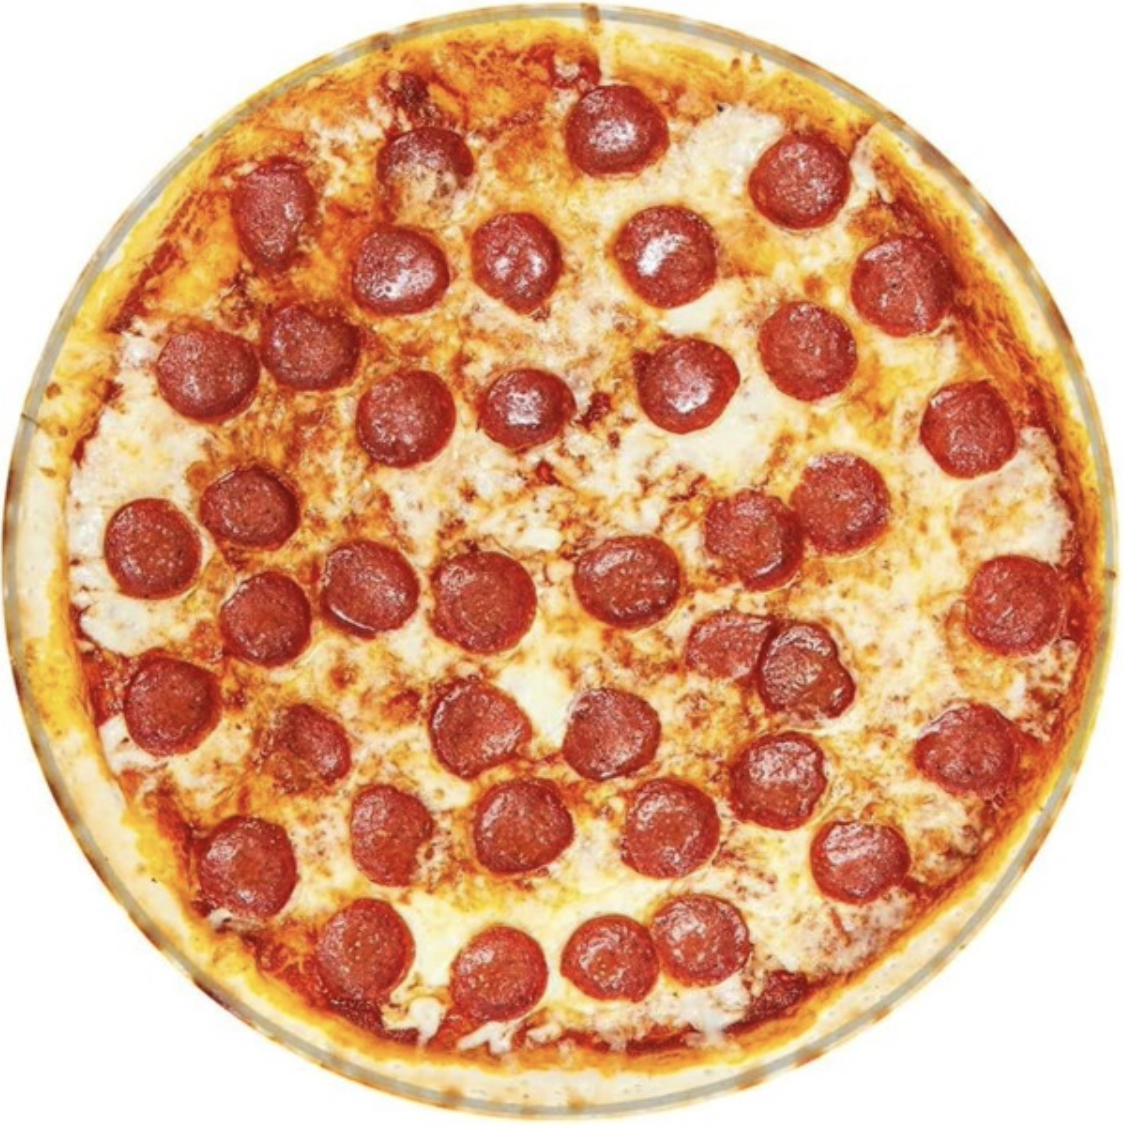
\includegraphics[angle=90,origin=c,width=1.2in]{pizza.jpg} 
   &
   \setbox0 = \hbox{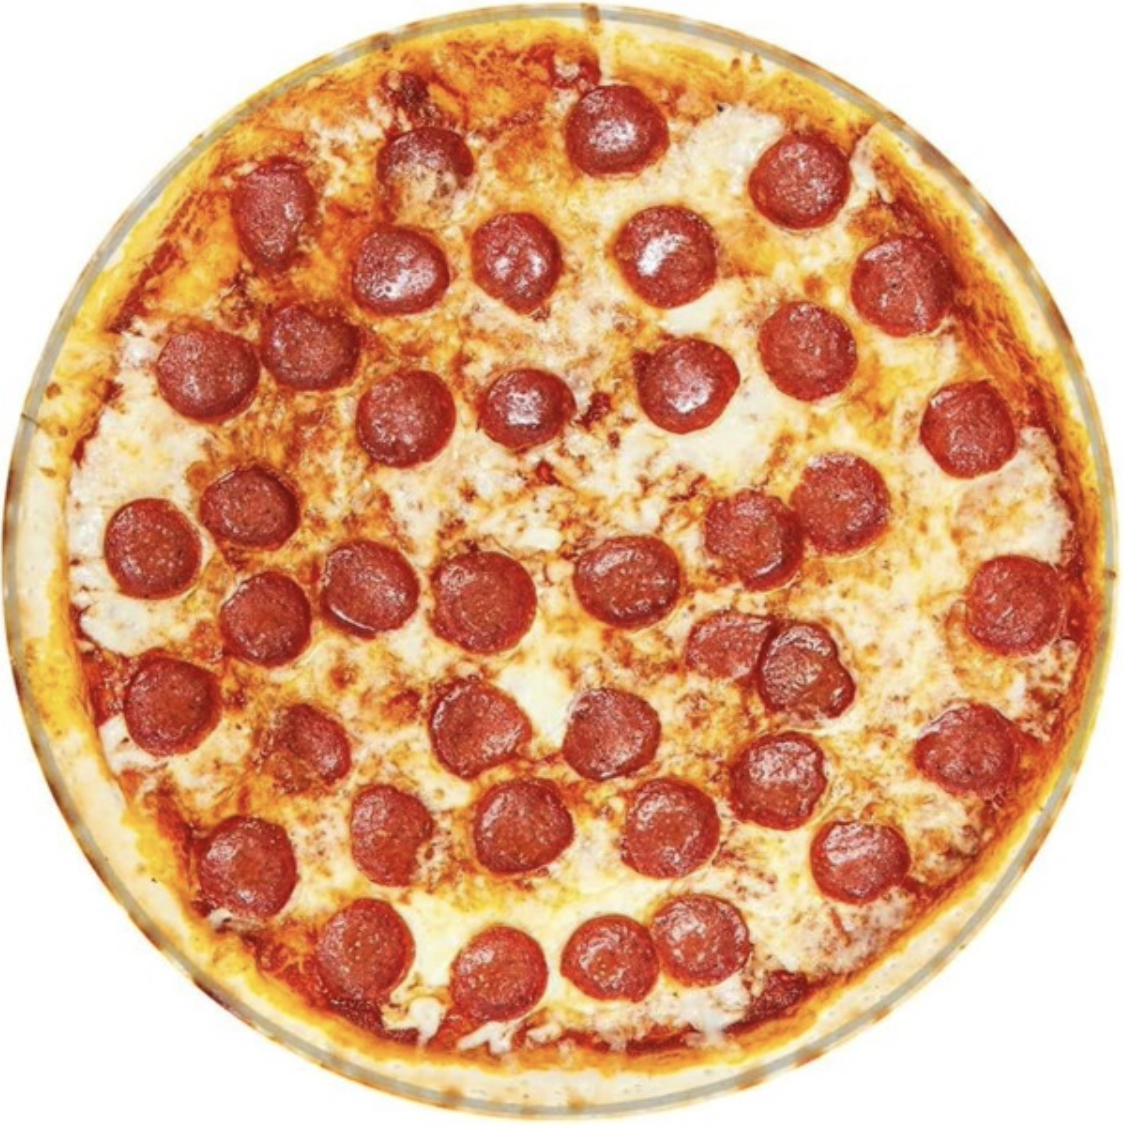
\includegraphics[width=1.8in]{pizza.jpg}}
   \setbox0 = \hbox{\lower 0.9in \copy0}
   \dp0 = 0in
   \copy0\\
   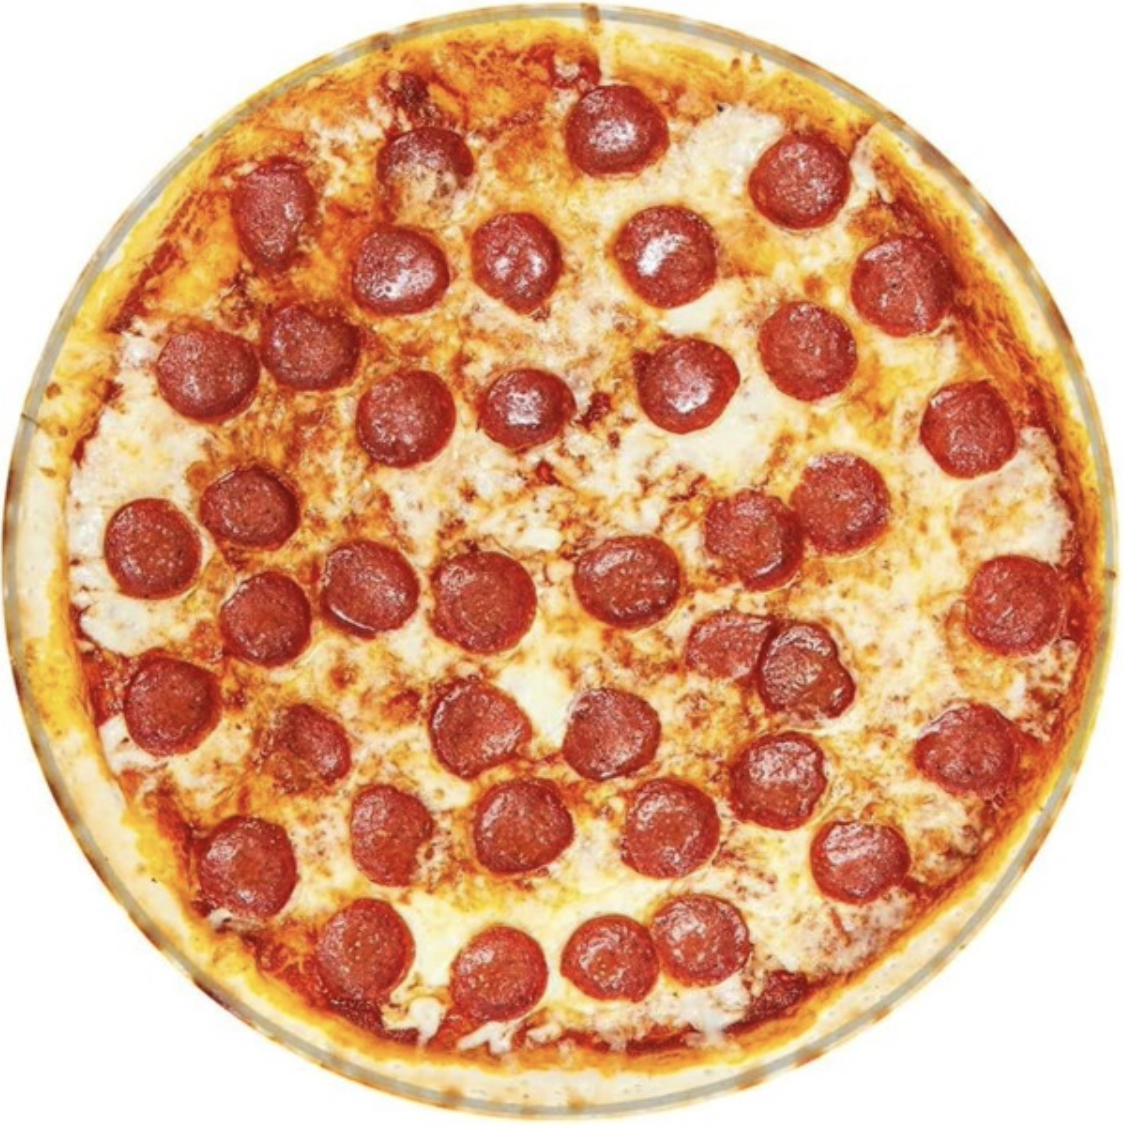
\includegraphics[angle=-90,origin=c,width=1.2in]{pizza.jpg}
   \end{tabular}
   \caption{If these two pizza orders (drawn to scale in the figure) are offered at the same price, does order \orderA\ or \orderB\ provide more food? (Figure based on figure 1 in \cite{pizzap}.)}
   \label{supplement-fig:pizzas}
\end{figure}

Now the choices are visualized in a figure, it seems clear that the question is intended to be: 

\begin{quote}\sf
If you can see or imagine two 12 inch pizzas offered for same the price as one 18 inch pizza (see figure \ref{supplement-fig:pizzas}), and you wish to buy the most pizza for the money, are you likely to correctly choose the greater amount of pizza and thus not be exploited by the pizzeria hoping to sell you less pizza for the same price?
\end{quote}

Evidently, the Pizza Problem raises non-trivial psychological issues, whether in vision or cognitive psychology, to say nothing of different people preferring crust and others a tomato-covered base, and so forth. Divertingly interesting as that may all be, the paper \cite{pizzap} in fact defines ``the pizza problem'' as the modeling issues that the problem succinctly illustrates, namely:

\begin{quote}\sf
Experience is seeing our ideas being executed by a computer, giving us the chance to debug scientific thinking in a very direct way. If we do not make our thinking explicit through formal modeling, and if we do not bother to execute (i.e., implement and run our specification through computational modeling), we can have massive inconsistencies in our understanding of our own model(s). We call this issue ``the pizza problem.''
\cite{pizzap}
\end{quote}

This is an insightful point, but there is much more to the Pizza Problem synecdoche than the paper suggests.

\section{Specifying and implementing the Pizza Problem}
The paper \cite{pizzap} proposes three elementary mathematical equations for a specification. Unprimed equation numbers are copied over from the original paper.

The amount of food $\phi$ per order $i$ is given as:

\begin{equation}\label{eqn-area}
\phi_i = N_i \pi R_i^2
\end{equation}

As defined above, $\phi_i$ specifies the total geometric area of $N_i$ pizzas all ordered with equal radius $R_i$. The formula has no visual or cognitive factors.

A decision rule is then given to specify the pizzeria order with most food:
\begin{equation}\label{eqn-specification}
\omega(\phi_i,\phi_j)=\left\{\begin{tabular}{ll}
$i$,& if $\phi_i>\phi_j$\\
$j$,&otherwise
\end{tabular}\right.
\end{equation}

This is incorrect, since if $\phi_i=\phi_j$ the biggest is not $i$ as in this case the orders $i$, $j$ have equal largest areas. The specification $\omega$ is also incorrect on the basis that the problem asks whether it is correct that the offer is a good deal; the answer to that question (whatever the question precisely may be, as discussed above) is a truth value not an order identifier. Notwithstanding that the formula has no psychological factors, nor any factors to disentangle the meaning of the question, one possible corrected definition of $\omega$ is: 

\begin{equation}\tag{$\ref{eqn-specification}^\prime$}\label{eqn-corrected-specification}
\omega(\phi_i,\phi_j)=\left\{\begin{tabular}{ll}
$i$,& if $\phi_i>\phi_j$\\
$\{i,j\}$,&if $\phi_i=\phi_j$\\
$j$,&if $\phi_i<\phi_j$\\
\end{tabular}\right.
\end{equation}

\def\psych{\overline{\phi}}
The set $\{i,j\}$ seems over-complicated as an answer to the Pizza Problem as posed. The actual meaning of $\phi_i=\phi_j$ is that both choices are of equal value to the customer, and the answer presumably is ``yes, that is a good deal,'' not a set. Something is not quite right. One solution is to introduce a psychologically-motivated version of $\phi$, say $\psych$, then a plausible formulation of $\omega$ would be

\def\order{\mbox{order}}
\begin{equation}\tag{$\ref{eqn-specification}^{\prime\prime}$}
\omega_{i,j}= \order(\psych_i, \psych_j) = \order(\phi_i,\phi_j)
\end{equation}

\ldots\ that is, the deal is a good one when the ordering of the participant's subjective assessment of the offer total areas is equal to the objective geometric ordering of the total areas --- that is, the participant is not fooled. This formulation implicitly raises the question of modeling a mental $\overline{\order}$, since a psychological representation of $\order(\psych_i, \psych_j)$ is implausible; and so forth.

Arguably, in the original paper then, an important benefit of computer modeling has been missed: developing a rigorous model specification (equation \ref{eqn-specification}) because correct computer code requires it has apparently not led to clarifying the problem specification itself.

A computational concern raised by equation (\ref{eqn-corrected-specification}) is that $\omega$, as specified, can only have a singleton value or a set (possibly multiset) of two values. Code that only handles a finite maximum number of cases (here, the maximum is 2) is likely to be unnecessarily restrictive. 

More general, and hence more robust, code will handle an unlimited number of cases. One such generalized specification of $\omega$ inspired by this scrutiny of equation (\ref{eqn-specification}) is as follows:

\begin{equation}\tag{$\ref{eqn-specification}^{\prime\prime}$}\label{eqn-set-corrected-specification}
\omega=\left\{i| \phi_i=\max(\phi)\right\}
\end{equation}

Note that this definition is `automatically' an empty set if there is no such $i$.

Equation (1) is subsequently generalized in \cite{pizzap} to allow different radius pizzas within a single order, as follows:
\begin{equation}\label{eqn-area-generalized}
\phi_i=\sum_{j=1}^N \pi R_j^2
\end{equation}

This is incorrect, since in equation (\ref{eqn-area}) $R_i$ was the radius of order $i$, not the radius of pizza $j$ in order $i$. The radius of pizza $j$ in order $i$ would be better written as $R_{i,j}$. 

The summation in equation (\ref{eqn-area-generalized}) is given over $N$, but since pizza orders --- as in the Pizza Problem itself --- may have different numbers of pizzas, it should be over $N_i$.

Hence a corrected form of equation (\ref{eqn-area-generalized}) is:

\begin{equation}\tag{$\ref{eqn-area-generalized}^\prime$}\label{eqn-corrected-area-generalized}
\phi_i=\sum_{j=1}^{N_i} \pi R_{i,j}^2
\end{equation}

In \cite{pizzap}, Python code is presented to implement $\phi$ as \texttt{food} (from equation \ref{eqn-area}), and anonymous code is then presented to implement $\omega$ (from equation \ref{eqn-specification}): 

\begin{verbatim}
# Decision rule (eq. 2): 
print(food(two_pizzas) > food(one_pizza))
\end{verbatim}

The code shown above yields a truth value, not $i$ or $j$ as actually specified by $\omega$ in equation (\ref{eqn-specification}). It happens to print \texttt{False}, but, even so, it does not meet the original English description of the problem as stated in the paper, since it does not address whether the offer is a good deal or not --- specifically, it calculates the truth value whether two 12 inch pizzas have a larger geometric area than one 18 inch pizza. 

Psychology is not modeled here. Participants may think or be misled (e.g., by an optical illusion) that two 12 inch pizzas represent more food than one 18 inch pizza, and if so they will be fooled and not choose a good deal. To answer the question posed, if they are fooled the correct calculated answer to the question should be \texttt{False}, which \emph{only coincidentally\/} is the same answer as the paper's Python calculation whether two 12 inch pizzas have a larger area than one 18 inch pizza --- the given code is only providing the right answer because it is answering the wrong question. 

Had the two pizza orders in the offer been of the same total area, the program would also have answered \texttt{False}, which in this case would be incorrect, since choosing either option would (on this assumption) have been an equally good deal. The answer the program provides is correct only because, again purely by chance, it was given data giving different areas. The code should have checked that the total areas were different since it relies on that assumption.

An interesting issue implicit in the paper's implementation is that the Python variables \verb|one_pizza| and \verb|two_pizzas| have values that are arrays of diameters of pizza orders (e.g., \texttt{[18]}, \texttt{[12,12]}), whereas the specifications for $\phi$ and $\omega$ both refer to identities of orders (e.g., $i, j$, etc). Arguably given the specification a programmer could legitimately choose that the implementation uses 1 or 2 (order numbers or other order identifiers) but \emph{not\/} the concrete details of the pizza diameters the specification has abstracted away, but which is what these Python variables denote. This point will be addressed below.

\section{A corrected implementation}
Python code implementing a corrected specification, equations (\ref{eqn-set-corrected-specification}) and (\ref{eqn-corrected-area-generalized}), is as follows. 

As a result of defining $\omega$ as a set in equation (\ref{eqn-set-corrected-specification}), the code now developed works with any number of orders, including zero orders and empty orders (both orders of zero pizzas and orders of pizzas of zero diameter). Note that this corrected implementation, like the original, is \emph{a\/} model of the problem, and like the original it fails to support any psychological interpretation of experimental data. Nevertheless there are still important observations to be reported here on the computational modeling process, regardless of such details.

We start with simple housekeeping to define the value $\pi$ for the program: 

{\tt\begin{tabbing}
import math\\

$\pi$ = math.pi
\end{tabbing}}

Next, we use a Python dictionary to define the mapping $\mbox{\it order} \mapsto \mbox{\it pizza-diameter}^{*}$, which is initialized with the given problem data. The dictionary, rather than the simple real-valued array variables as used in \cite{pizzap}, enables the corrected implementation to use the identifier of the greatest total area order(s) as defined in equation (\ref{eqn-set-corrected-specification}). This observation relies on an elementary but critical programming distinction resolved by Christopher Strachey in 1967 \cite{strachey}.

{\tt\begin{tabbing}
\# A map of Pizza orders\\
\# Variable orders[] maps order ID to a list of pizza diameters in inches\\ \\
orders = \{\\
\ \ \ \="\orderA": [12, 12], \=\# Order \orderA\ is two 12 inch pizzas\\
   \>"\orderB": [18] \>\# Order \orderB\ is one 18 inch pizza\\
\}
\end{tabbing}}

Note that Python will ignore if dictionary keys are repeated, so if this is a potential error it should be checked for independently of the implementation of the map shown above. If, for instance through a typo, they were both called \orderA, say, then Python would incorrectly, unfortunately without reporting any error, only assign one order to \texttt{orders[]}. In the case here there are only two orders and it is easy (but essential) to eyeball that they are correctly recorded in the Python code as two independent entries. 

Implementing the sum in $\phi$ is a routine matter of translating mathematics to Python idioms, noting the quite trivial conversion of diameters to radii as required by the mathematical definition of $\phi$:

{\tt\begin{tabbing}
\# Implement $\phi$ from (\ref{eqn-corrected-area-generalized})\\
\# Tota area of all pizzas in orderID\\
def phi(orderID):\\
\ \ \ \=totalArea = 0\\
   \>for diameter in orders[orderID]:\\
   \>\hskip 1em\=totalArea += $\pi$ * (diameter/2)**2\\
   \>return totalArea
\end{tabbing}}

Given the nature of the problem involving a low number of modestly-sized pizzas, no effort is made here to check for numerical over- or under-flow. (In general, numerical checking and other sanity checking should always be undertaken in case computer errors lead to incorrect results that are not flagged as such.)

Implementing $\omega$ is slightly more complex; for example, it is an obligation to prove that a Python list correctly implements the mathematical set $\omega$ in this case. Relevant details of the methodology used can be found in Dijkstra \cite{dop} and elsewhere in the standard computer science literature. Note that Dijkstra and others make it clear that the present paper just discussing a specification (and alternatives) and then presenting the resulting code has omitted a considerable body of mathematical reasoning that has had to be taken for granted to save space and patience. We will discuss this issue more comprehensively, below, in section \ref{section:pedantry}.

{\tt\begin{tabbing}
\# Implement $\omega$ from equation (\ref{eqn-set-corrected-specification}) \\
\# Determine maximum area order(s) over all orders\\
maxArea = 0\\
maxAreaIDs = []\\
for orderID in orders :\\
\ \ \ \=area = phi(orderID)\\
   \>if maxArea == area : \\
   \>\ \ \ \=maxAreaIDs.append(orderID)\\
   \>if maxArea < area  :\\
   \>   \>maxArea = area\\
   \>   \>maxAreaIDs = [orderID]
\end{tabbing}}

After the calculation above, the corrected result, allowing for the $\phi_i=\phi_j$ case and including empty orders, zero diameter pizzas, and multiple equal greatest total areas, can be obtained by writing

{\tt\begin{tabbing}
print(maxAreaIDs)
\end{tabbing}}

If English is preferred, the result can be formatted more understandably:

{\tt\begin{tabbing}
   
print\=(\="Pizza order", maxAreaIDs, \\
     \> \>"has largest area =", round(maxArea, 1), "sq in"\\
     \>)
\end{tabbing}}

To improve the English to cover the grammatically distinct cases when there are no orders, a single order, or when there is more than one greatest area order, the wording can be improved to depend straight-forwardly on \texttt{N} (implementing the specification $N=|\omega|$), the number of greatest orders:

{\tt\begin{tabbing}
N = len(maxAreaIDs)\\
if N == 0 : \\
\ \ \ \=print("No pizza orders were made")\\
else :\\
      \> print\=(\="Pizza", "orders" if N > 1 else "order", \\
	  \>      \>\>maxAreaIDs, "has" if N == 1 else "have equal",\\
	  \>      \>\>"largest area =", round(maxArea, 1), "sq in"\\
	  \>      \>)
\end{tabbing}}

If concerned (for instance to copy and paste the results into a paper we intend to publish) we could also improve the formatting of the value of \texttt{maxAreaIDs} in the print statement above. As written above, \texttt{maxAreaIDs} will appear in Python notation, not in English nor even in standard mathematical set notation. It is not hard to correct this shortcoming, but to do so would be a diversion from the thread of this paper.

The output of the program is now ``more'' than required by the specification, particularly equations (\ref{eqn-specification}) or (\ref{eqn-set-corrected-specification}): in addition to correcting bugs and using English to clarify the output, this code generalizes the original specification to additionally cover all cases $N \ne 2$, as well as providing the area of the order(s) with greatest area. (Python dictionaries cannot have $N<0$ elements, so necessarily $N\ge0$.) 

These generalizations are legitimate, since in general specifications logically imply correct code, so code can do more unless it is inconsistent with the specification. Note that a correct implementation of the specification has not resulted in code that provides a valid answer to the original question, because the question was not correctly specified.

Typically one would show that a projection of the code's output is implied by the specification, and one would provide an assurance case that the specification correctly captured the relevant essence of the original problem.\footnote{For an authoritative overview of assurance case practice, see \cite{assurance}.} Since in all but the simplest cases proving such an implication will be too demanding, critical parts of the code are generally constructed to be correct (so-called correct-by-construction, CBC) and an assurance case is separately made that the remainder of the code (for example, the user interface) does not affect the correctness of the required results. In the present case, for brevity, we omitted both details of constructing a correct implementation of $\omega$, as well as of the necessary testing.\footnote{Specification and refinement are subject to human error, but even if a specification and refinement to code are correct, programmers may make slips and introduce unnoticed errors in the coding process. Testing is essential to check correctness of implementations; furthermore, testing itself should be checked as it itself may contain unknown errors.} Curiously, testing correct grammatical English generation was more tedious than testing the implementation of $\omega$.

\section{Modeling the observed diverse preferences}
The specification and implementation are envisaged (in the paper's figure 2) to be part of an iterated serial process, being the middle two steps of six. In their scheme a cognitive framework (such as ACT/R \cite{actr}) comes first, and, notably, data comes last. Yet in their own discussion observed data of the Pizza Problem came first.

The modeling above shows that a correct rational ``algorithmic person'' preferring pizzas by area would consistently prefer option \orderB, as the program is clearly deterministic and produces the same result on every run. However, interest in the Pizza Problem was originally motivated by the observation of diverse answers to the question posed, thus motivating a psychological inquiry and building a model. The  code presented in \cite{pizzap} does not attempt to model the variation in the motivating data. One might then seek a more general model to explain the observed variation in participant preferences. 

For example, models based on a linear combination $\alpha \phi(t)+ (1-\alpha)[\phi(r)-\phi(t)]$, for pizzas radius $r$ with toppings radius $t$ ($t\leq r$), could be hypothesized to classify data from people preferring topping or crust. Other variables are the price (or expected price) of the pizza orders, and whether the participant is answering the verbal question ``looks larger'' (which implies visual introspection) or ``is larger'' (which more likely implies a geometric and purely cognitive question to the participant); or perhaps the question is asked illustrated with scale pictures, or even pizzas to both look at and smell. And so on.

To do any such modeling would require data, which is not provided in \cite{pizzap}.

\section{Is this pedantry?}\label{section:pedantry}
Is our discussion unnecessary pedantry about one paper's specification and code? Indeed, almost uniquely in this case, the original code in the paper \cite{pizzap} was merely an illustration of a methodology the paper proposed, and nothing in the paper really depended on the code actually being correct and doing what was claimed.

On the other hand, the original paper itself sets a very high standard of rigor: it argues that by providing an explicit computational model --- they mention using the formal methods $\mbox{TLA}^{+}$ \cite{tla} or Z \cite{z}, which are themselves very rigorous formal notations. Using such methods, in the authors' own words, they would debug scientific thinking.

Ironically, both the specification and code in the original paper are incorrect, and a human reader, given that both are trivial and arguably both just sketches, might choose to gloss over the errors as pedantry. One might note that the actual points about psychological modeling the paper is discussing superficially do not depend on the accuracy, correctness, or precision of either the specification or the code in the examples given. (That is, the model shown merely illustrates the arguments of the paper; it is not a direct model the running of which implies any substantial claims made in the paper.) Yet to gloss over rigor in this process would miss the opportunity to uncover that the problem has been inadequately specified and that even the simple implementation is incorrect. The implementation provides a superficially correct answer despite invalid reasoning. How can one debug scientific thinking that is not presented clearly, and, in the present case, is sufficiently vague to conceal incorrect calculations? Potentially the paper \cite{pizzap} has missed some critical steps in its proposed methodology? Indeed, the present paper has made various suggestions, including assurance cases, testing --- also leaving a lot of basic computer science unspoken --- all of which appeared necessary to get even the simple Pizza Problem to work sensibly.

The coding issues raised in the present paper will undoubtedly feel like pedantry for people who do a lot of programming without feeling they need to worry about formal computer science issues. 

Their code works. 

They think.

It is a difference in disciplinary perspectives. 

In my view, if you want to do coding, you may as well do it properly. Doing code properly is a rigorous discipline that leads to better and more dependable models and programs. It is important particularly if the code is critical, for instance perhaps for a psychology paper informing education or mental health interventions. Other papers criticized in \cite{harold-cj} used unreliable computer models to inform public health measures during the COVID-19 pandemic.

It is the same as an electrician `pedantically' pointing out that your extension lead needs an earth; they say it needs to be wired properly. You may well have a faulty extension lead without an earth that you have used successfully many times (musicians often remove the earth deliberately \cite{earthlift}, risking fatalities), so you think this is a pedantic demand over a trivial issue. Yet you are unnecessarily risking electrocuting yourself when doing the ironing or playing the keyboard. What is more, if you are playing with a band or in public [in the UK or EU], correct wiring is a legal requirement. An electrician's `pedantry' over a `trivial' issue will save somebody being killed, and will save you from a manslaughter conviction.

Can good music be based on sloppy wiring? Only by chance --- in that by chance you risk electrocuting a musician and having no music to listen to; by chance alone you hope the musician will not die. On the other hand, using proper professional wiring (e.g., earth bonding, protective devices, isolated supplies, extra low voltage supplies, etc) you can reduce the risk of electrocution to vanishing levels. Sadly, most of the time non-electrically qualified people cannot even tell the difference, and very likely they may not know how to tell the difference either. 

Can good science be based on sloppy code, and sloppily derived code from sloppy specifications? Only by chance. And who wants to rely on chance when you can do better? Why waste time --- why waste other people's time trying to read, understand, and develop your science --- by doing sloppy science.

\section{Consider a spherical cow \ldots}
A thought-provoking joke in physics begins ``consider a spherical cow \ldots'' Superficially it seems absurd, yet abstraction is a common, and productive modeling approach in any subject. In physics, a spherical cow has the same volume and mass as an actual cow-shaped cow, and can be used for many valid calculations,\footnote{For example, Isaac Newton showed that the $F=ma$ force acting on any body of any shape was the same as if that body was mathematically reduced to a point mass (of the same mass) placed at the center of gravity of the body. In fact, the rigorous concept of center of gravity is precisely a spherical cow (or anything) of the same mass and radius zero.} yet has abstracted away complicated details of real cows that would make modeling impractical. The point is, where the abstraction works it is very valuable and the nature of the abstraction allows its validity to be quantified. For example, if you want to spin a cow, the angular momentum of a sphere and a cow are different, but a sphere's angular momentum can be used to approximate it, perhaps adequately for the purpose.

Is a model such as that used in \cite{pizzap} a ``spherical cow''? 

The mathematical model is, as it is precise and abstracts away complicated details (such as cognitive issues) --- and this is very clear in \cite{pizzap}. The computational model, however, is not; the way in which it abstracted details (by implementing the mathematics) is unknown because it has bugs that undermine the validity of the abstraction, as described above.

The problem is that the refinement from the mathematical specification (equations 1--3) is tedious. Even the present paper omitted it, and referred to standard textbooks. Furthermore, it is error-prone, and considerable skill is required to assure the final computational model is correct (or correct enough).

Alternative approaches are possible, and in general are essential to ensure the quality of the science. For example Alloy \cite{alloy} is a specification language (with practical and comprehensive computer support) that allows an abstract specification to be incrementally refined. An Alloy specification can start closer to the pizza problem than the equations in \cite{pizzap} and corrected here, and it can include cognitive factors. How it is then refined is a matter for the scientist. The book \cite{alloy} also reviews other methods that may be more or less appropriate to other modeling problems.

\section{Conclusions}
This paper has shown that the Pizza Problem is a productive idea, though it is noteworthy for being simple enough to identify and address unintentional errors. Unfortunately, almost all scientific modeling is far more complex and is, one would assume, very likely to be incorrect in more subtle and less unconstructive ways.

In general, then, modeling is complex. Minor errors, such as those exhibited in the original paper \cite{pizzap}, are rarely obvious. To debug scientific thinking reliably, models need to be correct (or as correct as reasonably possible) relative to proposed specifications in the first place. We would argue that not only sharing specification and code is necessary, but a methodological step of ``assuring correctness'' is also necessary and needs to be done competently. Assuring correctness should be included in a paper's proposed methodology pathway.

\emph{Availability of code}. The Python code in this paper was extracted directly from the source \LaTeX\ by a simple \texttt{awk} script, and then run using Python version 3.9. The code is generated and run using a simple \texttt{make} file. In other words, the code presented in this paper as typeset has been checked to work as described.

\emph{Acknowledgements}
With thanks to Peter Ladkin and the authors of \cite{pizzap}, Olivia Guest and Andrea Martin, who commented on this paper and raised the spherical cow analogy.

\begin{thebibliography}{99}

\bibitem{actr}
Anderson, J. R. \emph{Rules of the Mind}, Erlbaum, 1993.

\bibitem{dop}
Dijkstra, E. W. \emph{A Discipline of Programming}, Prentice Hall, 1976.

\bibitem{pizzap}
Guest, O. \& Martin, A. E. ``How computational modeling can force theory building in Psychological Science,'' \emph{Perspectives on Psychological Science}, \textbf{16}(4):789--802, 2021. DOI 10.1177/1745691620970585

\bibitem{alloy}
Jackson, D. \emph{Software Abstractions}, MIT Press, revised edition, 2012.

\bibitem{assurance}
Knight J. C.,  Rowanhill, J. \& Rinehart, D. J. \emph{Understanding What It Means for Assurance Cases to ``Work,''}
NASA/CR–2017-219582, National Aeronautics and Space Administration
Langley Research Center, 2017.

\bibitem{tla}
Lamport, L. \emph{Specifying Systems: The TLA+ Language and Tools for Hardware and Software Engineers}, Addison-Wesley Professional, 2002.

\bibitem{z}
Spivey, J. M. \emph{Z Notation: A Reference Manual}, Prentice Hall International Series in Computer Science, 1992.

\bibitem{strachey}
Strachey, C. ``Fundamental concepts in programming languages,'' republished in \emph{Higher-Order and Symbolic Computation}, %Kluwer Academic Publishers, 
\textbf{13}(1/2):11--49, 2000. DOI 10.1023/A:1010000313106

\bibitem{heedless}
Thimbleby, H. ``Heedless programming: {I}gnoring detectable error is a widespread hazard,'' \emph{Software --- Practice {\&} Experience}, \textbf{42}(11):1393--1407, 2012.
DOI 10.1002/spe.1141

\bibitem{harold-cj}
Thimbleby, H. ``Improving science that uses code,'' \emph{Computer Journal}, in press.

\bibitem{earthlift}
Wikipedia, ``Ground Lift,''
\url{https://en.wikipedia.org/wiki/Ground_lift#cite_note-self06-1}, viewed 2023.

\end{thebibliography}

\end{document}

\section{New issues created by computer modeling}
A scientist would iteratively experiment, theorize, calculate, and write up their research. Although final papers are often written up in a structured way, there was little to constrain the process of science itself. Now, with computers, the additional steps of specification, programming, calculating (e.g., for statistics results) and executing computer models have been introduced --- along with using computers to support the writing processes.  

In general, specification, programming, and running models can be done in any order, revised and iterated as corrections and new ideas are considered. However, at least for writing up, it is convenient to simplify the reality to a linear process: problem statement $\sqsupseteq$ specification $\sqsupseteq$ implementation $\sqsupseteq$ execution. The symbols $\sqsupseteq$ represent \emph{refinement}, with an abstract idea (on the left) related to its refinement into a more concrete form (on the right). Computer scientists are interested in how $\sqsupseteq$ works and how to support it with automatic tools; for instance $\sqsupseteq$  is transitive (if $u\sqsupseteq v$ and $v\sqsupseteq w$ then $u\sqsupseteq w$), but this theory and tool support is beyond the scope of this paper.

The paper \cite{pizzap} uses the word \emph{specification\/} to refer to a phase in programming, namely defining how a model should work. Interestingly, their discussion is itself a specification, a specification of psychological modeling.

Thus equation (\ref{eqn-corrected-area-generalized}) above, $\phi_i=\sum_{j=1}^{N_i} \pi R_{i,j}^2$, is more abstract than its refinement to the Python code that implements it. The Python code will necessarily introduce concrete details that are not in the specification, either because the specification permits it, Python or the programmer requires it, or because an error has been made. Thus, in the code given in \cite{pizzap}, there is nothing that correctly refines $\phi_i$ in equations (\ref{eqn-area} or \ref{eqn-corrected-area-generalized}); the parameter for \texttt{food} is the refinement of $R_i$ not $i$. Confusingly, the Python in \cite{pizzap} uses variable names (\verb|one_pizza| and \verb|two_pizzas|) to refine $R_i$, but these are names that are not values in the model --- the Python code loses the specification variable $i$. The model --- the running program --- represents two possible values of $R_i$, but it does not represent $i$ itself, and the concept of subscripting $R$ has been lost. (This paper's Python instead used a dictionary to represent pairs $(i,R_i)$ together as explicit program values.) 

Given that these different refinements are legitimate, it is clear that the given specification has \emph{under-specified\/} the code; here, how an order is represented is has not been explicitly specified, and therefore it has been left open to interpretation. An easier to understand under-specification is that the programming language was not specified, leaving it open to the programmer to make any choice, and, presumably, using any programming language that can refine the equations would be acceptable.

Conversely, a specification may \emph{over-specify\/} the code. For example it might be specified that a customer's order called $x$ be represented by a variable called $x$. In \cite{pizzap}, the paper calls the orders \orderA\ and \orderB\ but the Python code happens to call them \verb|two_pizzas| and \verb|one_pizza| respectively.

  